\documentclass[11pt]{article} 
\usepackage{geometry}
\geometry{letterpaper}

\usepackage{graphicx}   
\usepackage{amssymb}
\usepackage{float}
\usepackage{tabularx}
\usepackage{framed}
\usepackage{hyperref}
\hypersetup{
    colorlinks,
    citecolor=black,
    filecolor=black,
    linkcolor=black,
    urlcolor=black
}
\usepackage{cleveref}
%\usepackage[autostyle]{csquotes}
\usepackage[english]{babel}
\usepackage[backend=biber,style=numeric,sorting=none]{biblatex}
\addbibresource{cites.bib}

\defbibheading{bibliography}[\refname]{}

\begin{document}

\newcommand{\PROJECTNAME}{SwarmBot}

\begin{titlepage}
	\newcommand{\HRule}{\rule{\linewidth}{0.2mm}}
	\begin{center}
	\textsc{\LARGE McMaster University}\\[1.5cm]
	
	\textsc{\Large \PROJECTNAME}\\[0.5cm]
	\textsc{\large Software \& Mechatronics Capstone}\\[0.5cm] 

	\HRule\\[0.4cm]
		{\huge\bfseries Requirements Document}\\[0.4cm]
	\HRule\\[0.4cm]
	
	\begin{minipage}[t][][t]{0.5\textwidth}
		\begin{flushleft} \large
			\emph{Authors:}\\
			Victor Velechovsky \\
			Amandeep Panesar \\
			Taha Mian \\
			Gabriel Potter \\
			Nishanth Balamohan \\
		\end{flushleft}
	\end{minipage}
	~
	\begin{minipage}[t][][t]{0.4\textwidth}
		\begin{flushright} \large
			\emph{Professor:} \\
			Dr. Alan Wassyng \\[0.4cm]
			\emph{Teaching Assistants:} \\
			Nicholas Annable \\
			Joshua Barkovic \\
			Spencer Deevy \\
			Viktor Smirnov
		\end{flushright}
	\end{minipage}\\[2cm]
	
	
\includegraphics[width=0.3\textwidth]{images/logo.png} \\
	{\large Last compiled on \today}
	\end{center}

\end{titlepage}

\tableofcontents
\listoffigures

\vfill
\begin{figure}[htbp]
   \centering
   \noindent\begin{tabularx}{\textwidth}{| >{\centering\arraybackslash}m{0.2\textwidth} | >{\centering\arraybackslash}m{0.2\textwidth} | >{\centering\arraybackslash}m{0.2\textwidth} | >{\centering\arraybackslash}m{0.285\textwidth} |}
   \hline 
   \textbf{Date} & \textbf{Revision} & \textbf{Comments} & \textbf{Author(s)} \\
   \hline
   Oct 28/2018 & 0 & Basic template & All authors\\ \hline
   Oct 29/2018 & 1 & Functional Requirements Added & All authors\\ \hline
   Oct 30/2018 & 2 & Other sections added & All authors\\ \hline
   Oct 31/2018 & 3 & Final draft for Requirements Deadline & All authors\\ \hline
   Mar 6 /2019 & 4 & Revision 1 & All authors\\ \hline
   \end{tabularx}
   \caption{Revision History}
\end{figure}

\newcommand{\functionalRequirement}[7]{
\begin{framed}
	\noindent\textbf{Requirement ID}: F{#1} \hfill \textbf{Requirement Type}: Functional \hfill\\\\
	\noindent\textbf{Description}: {#2} \\
	\textbf{Rationale}: {#3} \\
	\textbf{Fit Criterion}: {#4} \\
	\textbf{Originator}: {#5} \\
	\textbf{Priority}: {#6} \hfill \\
	\noindent\textbf{History}: {#7}
\end{framed}
}

\newcommand{\nonFunctionalRequirement}[7]{
\begin{framed}
	\noindent\textbf{Requirement ID}: NF{#1} \hfill \textbf{Requirement Type}: Non-Functional \hfill\\\\
	\noindent\textbf{Description}: {#2} \\
	\textbf{Rationale}: {#3} \\
	\textbf{Fit Criterion}: {#4} \\
	\textbf{Originator}: {#5} \\
	\textbf{Priority}: {#6} \hfill \\
	\noindent\textbf{History}: {#7}
\end{framed}
}

\newpage
%THIS DOCUMENT MUST INCLUDE
%-Scope
%-Context Diagram showing boundaries---???
%-Monitored and controller variables (with units)
%-Constraints
%-Behavior overview including notation---???
%-Diagrams showing functional decomposition---???
%-Required behavior description (keep away from design as much as possible)
%-Rationale where necessary - includes simulation analysis if you have any
%-Performance requirements
%-Normal operation (optional if handled in requirements with undesired event handling)
%-Undesired event handling(optional if handled in requirements with normal operation) --- ???
%-List of requirements that are likely to change
%-List of requirements that are not likely to change ---???
%-References

\section{Introduction}

There are many applications for carrying out distributed measurements over large areas. Analysis of irradiated areas, elevation mapping, and air toxicity measurements are among many. Unfortunately, it is both expensive and time-consuming to carry out such measurements over large regions. It typically requires many measurement stations, all placed in discrete locations, in order to provide accurate readings over large areas. We propose a fundamentally different approach.

\subsection{Project Overview}

\PROJECTNAME \space is a \hyperref[sec:definitions]{swarm} of autonomous robotic cars meant to carry out measurements over large areas. For our project, these cars will be measuring temperature, but the idea can be expanded to any number of other quantifiable measurements. Central to our work will be two major components. First, a small motorized car, attached with a temperature sensor, as well as a control unit that allows it to communicate with – and be controlled by – a centralized control unit. Second, a software package that can control a large group (\hyperref[sec:definitions]{swarm}) of these cars, with an algorithm focused on producing reliable, accurate, and fast measurements.\\

Our swarm will aim to cover large areas more quickly and cost-effectively than traditional products. To test the applicability of our project, we will demo it in a small scale area as well as develop a simulation to hypothetically prove the efficacy of the system on a larger scale.\\

Our project will be conducted between Fall 2018 – Winter 2019 for our Engineering Capstone project at McMaster University, under the guidance of Dr. Alan Wassyng. We have four Software Engineering students, and one Mechatronics Engineering student.

\subsection{Naming Conventions and Terminology}

\label{sec:definitions}
\begin{itemize}
\item \textbf{System}: The entire software and hardware package - including the cars,
car hardware, control software, and server running the control software
\item \textbf{Swarm}: A large group of objects (in our case, motorized cars) that can communicate and perform acts as a group
\item \textbf{Insect}: A member of the swarm (in our case, a single motorized car)
\item \textbf{Simulation}: The simulation will be used for demo purposes, mainly to show that
the system is valid with a large number of insects.
\item \textbf{Researcher}: A user that is interested in the data that is returned from the survey.
\item \textbf{System Administrator}: A user that controls the parameters of the \hyperref[sec:definitions]{\textbf{swarm}}.
\item \textbf{G.P.S.}: Global Positioning System
\item \textbf{Map}: A 3D visualisation of the data collected by the system.
\end{itemize}

\subsection{Relevant Facts and Assumptions}

For demo purposes, our project will be conducted on a small scale. One major assumption is that this project can be effectively expanded to a much larger scale – that of forests, fields, and larger geographic regions. There will likely be design challenges involved in a large-scale project, but due to the time and resources available to us, we must assume that such challenges could be overcome without compromising its fundamental goals. This assumption carries with it some implicit ones. Namely, we must assume that a large scale version of our project will be able to withstand the wind and otherwise adverse weather conditions of large geographic regions. It will need to be able to communicate reliably over much larger distances.\\

Another assumption we must make is that there are no sensitive lifeforms or other objects that can be harmed by the system, in the near vicinity of the system. An object collision detection algorithm can certainly be implemented, most likely using cameras and computer vision, but due to time constraints, we may not be able to include one. We will ensure the lack of sensitive lifeforms by inspecting the
(very small) coverage area prior to running the system.

To simplify the development and testing process, we will assume that weather conditions are as follows:

\begin{itemize}
    \item Air temperature between $10^o (C)$ and $30^o (C)$
    \item Air humidity between $10\%$ and $20\%$
\end{itemize}

\section{Project Drivers}
\subsection{Purpose}
The collection of data for the purpose of studying large areas poses the following problems: 
\begin{itemize}
    \item Measurements can vary substantially over the area of interest
    \item Measurements can vary substantially over time
\end{itemize}

Therefore, it is optimal to survey multiple test points spanning the area of interest and to collect data regarding the change in environmental conditions at those test points over a given time interval. The typical solution to this is to place sensors on fixed measurement devices and fix them to strategic locations. There are two main drawbacks to this approach:
\begin{itemize}
    \item The number of test points is limited to the number of fixed test points, which cannot be permanently placed in areas which will obstruct traffic (from humans or other life)
    \item The measurement tools cannot be reused in other areas
    \item Placing measurement devices in fixed, arbitrary locations can be costly and time-consuming
\end{itemize}

A possible solution to these issues is a robot swarm of measurement cars. These could be reused in many different regions, and because they are not permanently fixed they could potentially cover a wider range of test points. In addition, the mobility of the swarm allows test points to be measured in different parts of a region at different times, and as such more data can be collected with less equipment. Therefore, the purpose of this project is to build such a system.

\subsection{Key Stakeholders}
\subsubsection{Users}
The intended users of this system are primarily researchers requiring data for environmental analysis. This includes meteorologists, environmental scientists, biologists, among many others.
\subsubsection{Development Team}
The development team is responsible for both the project concept and its implementation. This will be done with the guidance of Dr. Alan Wassyng and his teaching assistants.
\subsubsection{Faculty}
McMaster University - specifically, the Department of Computing and Software - is invested in the success of this project. Upon successful completion, it can be used to highlight the quality of the program, department, and institution.

\section{Project Scope and Goals}
\subsection{Feasibility}
Due to time and financial constraints, defining the project's scope is essential to ensure the project is feasible. One way to ensure the project remains in scope is to restrict the area of the survey. Insects can travel only a maximum distance (approximately covering the size of a swimming pool) from the starting point. The test environment will also be level and free from obstructions. We will take advantage of third-party chassis systems, and will not be building our own. We will also rely on other third-party components, such as embedded micro-controllers and transceivers.

\subsection{Sensor Choice}
Another way we will reduce the scope of the project is by limiting the type of data we collect with each insect. While this system could be used with a multitude of measurement types, for this prototype we will limit our integration efforts to just two types. We have chosen to focus on temperature and humidity measurements for the following reasons:

\begin{itemize}
    \item Transmitting temperature/humidity information is akin to transmitting any other type of measurement -- the main control unit can be designed without regard for the type of data being collected
    \item Temperature/humidity sensors are relatively cheap in comparison to other measuring devices such as Geiger counters
    \item Heat is infrared radiation [\hyperref[sec:references]{1}] and therefore mapping it will be analogous to mapping other types of radiation (a possible usage scenario)
    \item Humidity is the water content of the air and therefore is analogous to other measures of air composition such as the amount of pollutants present (another possible usage scenario)
\end{itemize}

\subsection{Project Goals}
With the above scope considerations in mind, the following sections cover the necessary and optional goals for the project.
\subsubsection{Necessary Goals}
\begin{itemize}
    \item Measure the temperature and humidity of a small area (for demo purposes, approximately the size of a small swimming pool) as it varies by location and time
    \item Produce a visual representation of the measurements
    \item Produce a simulation to show the system working efficiently with a large number of insects in a larger area (for demo purposes) 
    \item Make the system flexible with respect to how many insects are in a swarm, so that end users can use as many/few insects as they want
\end{itemize}

\subsubsection{Optional Goals}
\begin{itemize}
    \item Explore other types of measurements and incorporate them along with the temperature and humidity measurements (or replace them, if need be). One possible idea for this is measuring air pollutant levels.
    \item Make the system as easy to use for a beginner as possible 
    \item Include object collision detection in order to improve safety 
    \item Design the boats to be as cost efficient as possible for end users 
    \item Create a phone app for end users to run the swarm from
\end{itemize}

\subsection{Individual Use Cases}

The actors that interact with the system are the \textbf{\hyperref[sec:definitions]{researcher}}, and the \textbf{\hyperref[sec:definitions]{system administrator}}. The researcher is a primary actor, and the system administrator is a secondary actor. The researcher does not have to be present during the operation of the system. \\\\
The following are the primary use cases:

\begin{itemize}
    \item \textbf{Researcher requests a specific area to be surveyed}:\\
        The initial state going forward with this action would be the insects are already placed in the area of survey, and have been paired to the server. The researcher has a particular area he wants to investigate. He will input this area into the GUI so that the software knows about the coverage area that he wants to inspect.Once the area coverage has been set the outcome is the insects begin to survey the area. 
    \item \textbf{Researcher analyzes the returned data}:\\
        The initial state for this use case is that the insects have all returned to the initial starting point and have reported back their findings.The outcome is data returned by the system is presented to the researcher in the form of a visual graph. For example, humidity information about the environment could influence decisions in land surveying.
    \item \textbf{Researcher requests to end surveying session}:\\
        Initial state for this scenario would be that the insects are in the process of conducting a survey. The researcher then stops the current survey which might be due to the fact enough data has been collected. The outcome is all the insects return to the initial starting point, and whatever data was collected is returned to the graphical interface. 
    \item \textbf{Researcher checks the progress of the survey}:\\
        The initial state of this use case would be that a survey is currently being conducted. The researcher then wants to know how much progress has been made in covering the coverage area, so through the GUI he checks what percentage of regions have been explored and measured by the swarm.
\end{itemize}

The following are secondary use cases:

\begin{itemize}
    \item \textbf{System Administrator sets the constraints of the survey}:
        The constraints of the survey would include the coverage area and the number of
        insects in the swarm. The administrator would make these changes through the GUI.
    \item \textbf{System Administrator deploys the swarm. This is done through the GUI.}:
        The swarm constraints have been set, so the administrator begins the surveying process.
    \item \textbf{System Administrator ends the session}:
        The administrator has detected an issue with the surveying process, such as a safety risk,
        so he ends the process prematurely, through the GUI.

\end{itemize}
\begin{figure}[H]
   \centering
   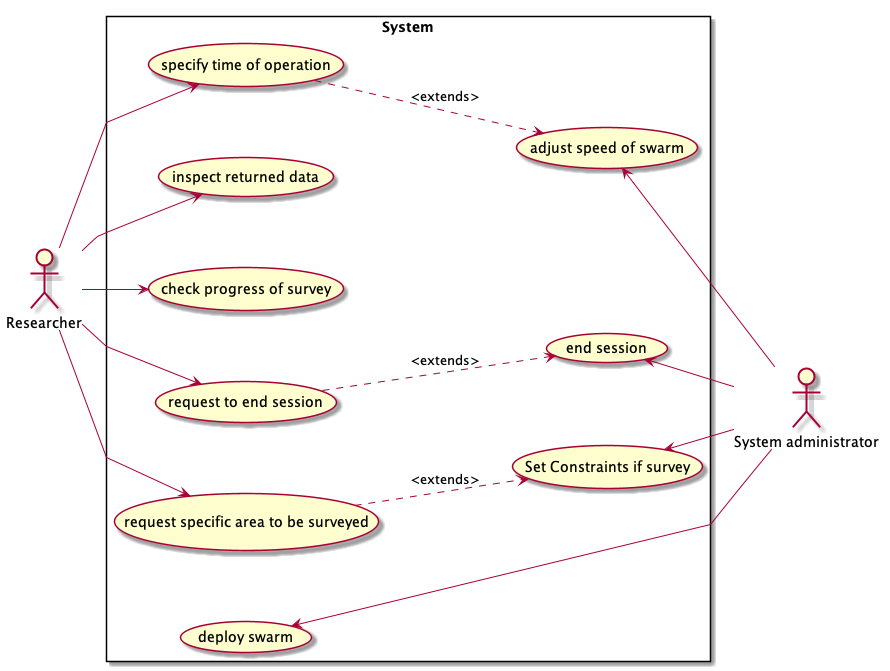
\includegraphics[width=\textwidth]{diagrams/usecase.png}
   \caption{Use Case Diagram}
   \label{fig:ucd}
\end{figure}

\subsection{Mandated Constraints}
There are 2 constraints put on the project. The first being time, since the project is due at the end of April 2019. The second constraint is money. There is a \$750 budget for this project.
\subsection{Undesired Behavior}
An insect should not lose connection to the server during the survey. An insect should not be hit or come in the path on any object including other insects. The power supply of an insect should not explode. The environment should not interfere with the operations of an insect. Other network signals should not interfere with the server and the swarm. 
\subsection{Variables}
\begin{figure}[H]
   \centering
   \noindent\begin{tabularx}{\textwidth}{| >{\centering\arraybackslash}m{0.2\textwidth} | >{\centering\arraybackslash}m{0.2\textwidth} | >{\centering\arraybackslash}m{0.2\textwidth} | >{\centering\arraybackslash}m{0.285\textwidth} |}
   \hline 
   \textbf{Variable Name} & \textbf{Type} & \textbf{Value} & \textbf{Description} \\
   \hline
   Area of survey & Fixed & $X$ in $m^2$ & The total surface area of coverage area in a survey \\ \hline
   Perimeter of survey & Fixed & $X$ in $m$ & The region that bounds the survey area \\ \hline
   \hyperref[sec:definitions]{Insect} location & Monitored & (X, Y) representing lat/lon values, respectively & The perceived location of an insect at any given time\\ \hline
   Temperature & Monitored & $X$ in $^\circ$C & The measurement an insect takes at a specific point\\ \hline
   Speed of  \hyperref[sec:definitions]{Insect} & Controlled & $X$ in $m/s$  & The speed relative to the ground of an insect \\ \hline
   Number of \hyperref[sec:definitions]{Insect} & Controlled & $X$ amount of insects & The number insects currently deployed in a swarm\\ \hline
   Battery life & Monitored & $X$ in $minutes$ & The amount of battery left in a specific insect \\ \hline
   Range of communication & Fixed & $X$ in $m$ & The range in which server can communicate with each insect \\ \hline
   Max Time for survey & Fixed & $X$ in minutes & The maximum time the survey will run for\\ \hline
   Min Time for survey & Fixed & $X$ in minutes & The minimum time the survey will run for \\ \hline
   Start Point & Fixed & (X, Y) representing lat/lon values, respectively & The Starting point from where an insect is deployed \\ \hline
   \end{tabularx}
   \caption{List of Variables}
\end{figure}

\subsection{Context Diagram}
\begin{figure}[H]
   \centering
   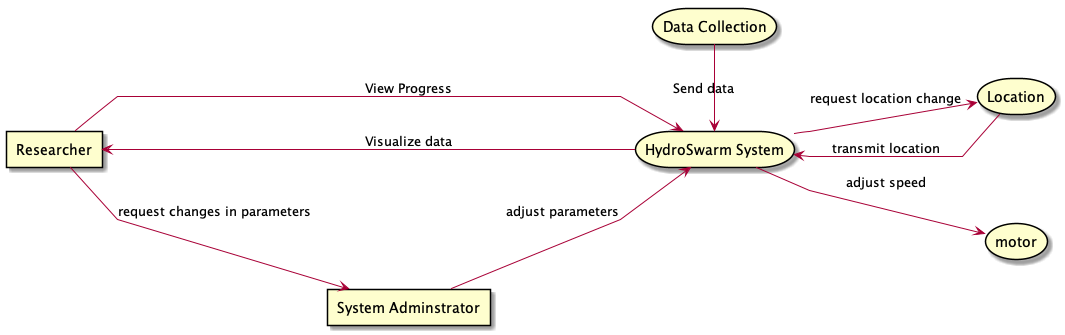
\includegraphics[width=\textwidth]{diagrams/context.png}
   \caption{Context Diagram}
   \label{fig:cd}
\end{figure}

\section{Functional Decomposition Diagram}
\begin{figure}[H]
   \centering
   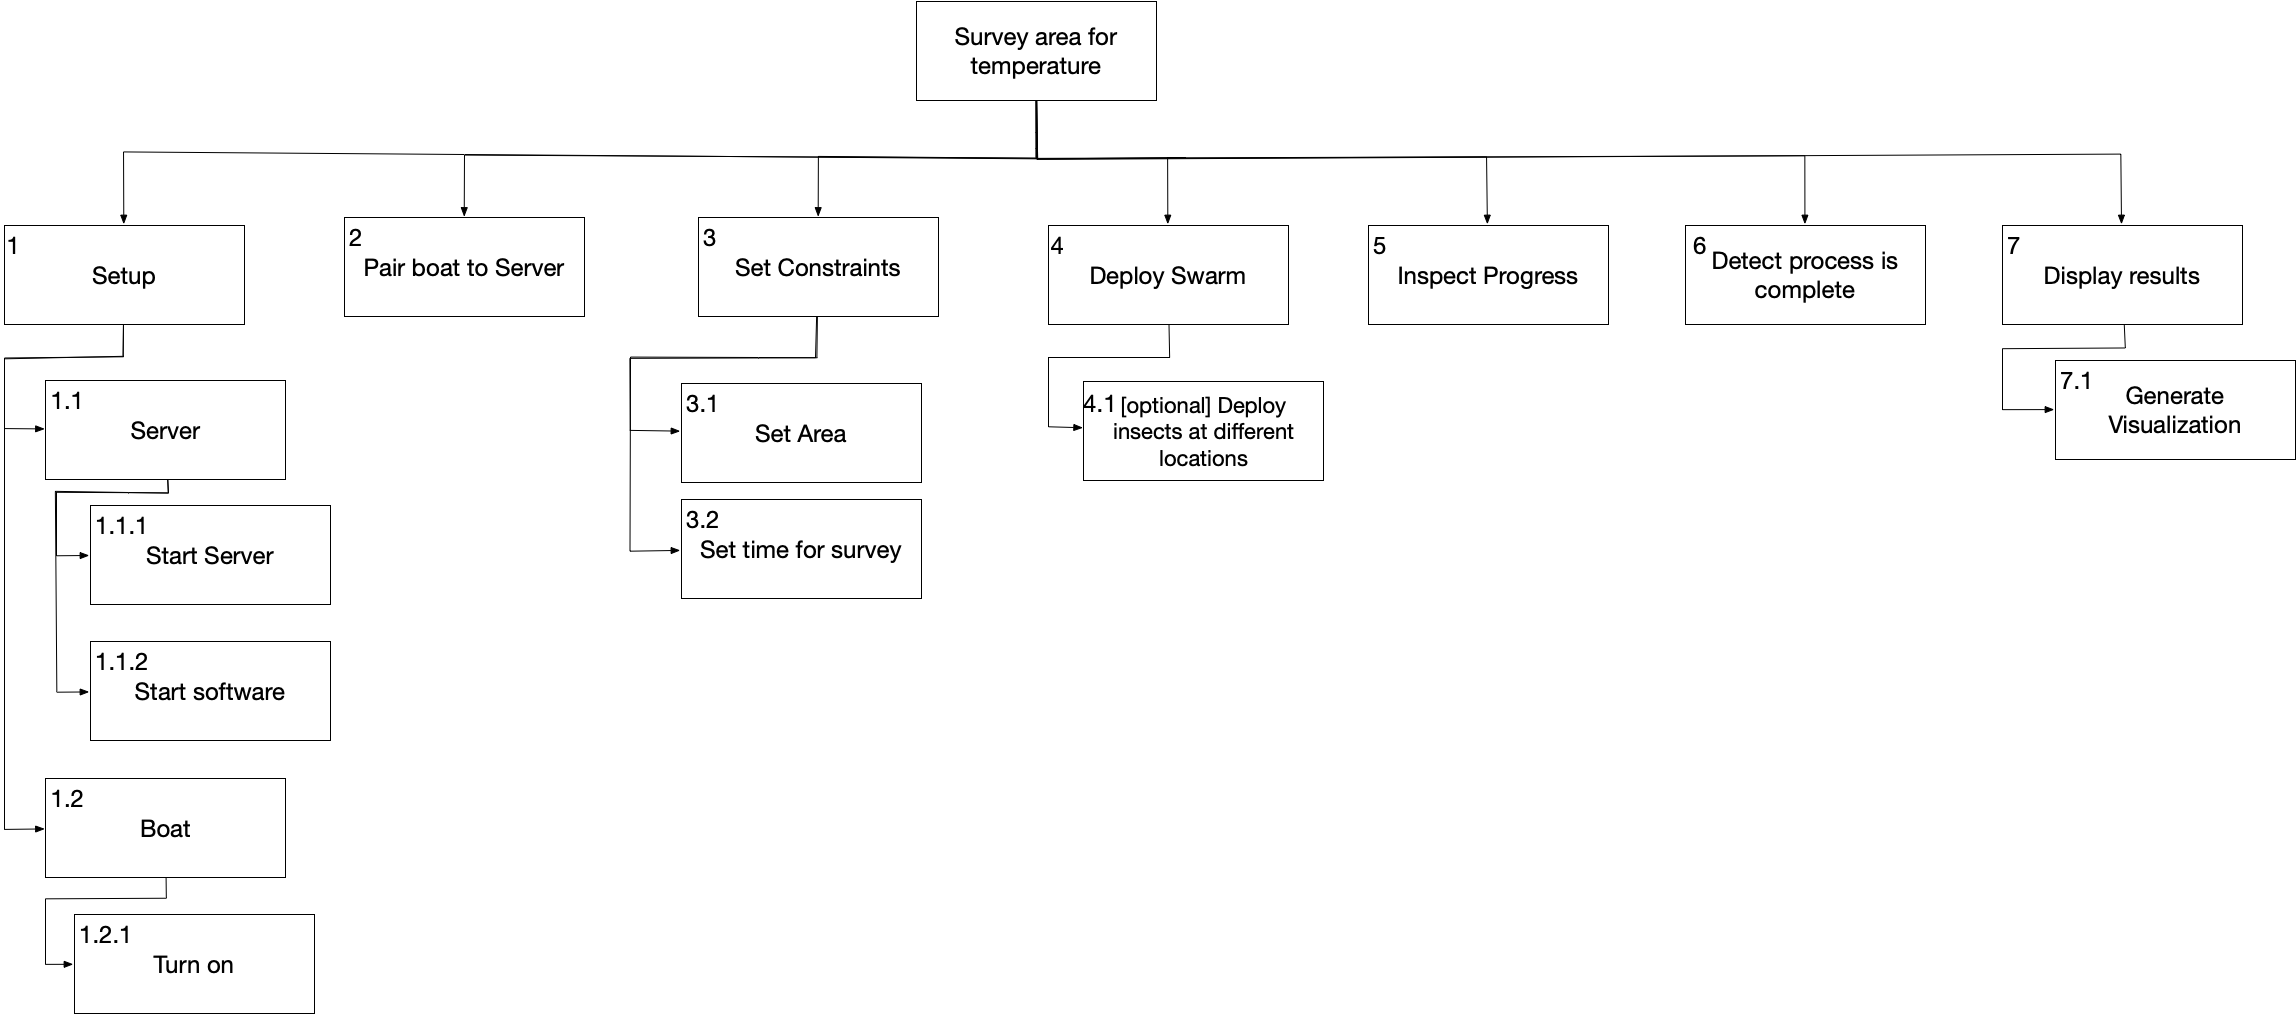
\includegraphics[width=\textwidth]{diagrams/functionaldecomp.png}
   \caption{Functional Decomposition Diagram}
   \label{fig:fdd}
\end{figure}

\section{Functional Requirements}

\functionalRequirement
{1}
{Each \hyperref[sec:definitions]{insect} in the
\hyperref[sec:definitions]{swarm}
must be able to measure
the air temperature at its current location}
{Accurate air temperature measurements have many applications
in academic or professional work}
{Each insect must be able to measure the air temperature accurately at its location
to within \pm $ 1^o C$ at all times}
{Victor Velechovsky}
{High}
{Created Oct. 28, 2018}

\functionalRequirement
{2}
{Each \hyperref[sec:definitions]{insect} in the
\hyperref[sec:definitions]{swarm}
must be able to measure
the air humidity at its current location}
{Accurate air humidity measurements have many applications
in academic or professional work}
{Each insect must be able to measure the air humidity accurately at its location
to within \pm $ 1^o C$ at all times}
{Victor Velechovsky}
{High}
{Created Oct. 28, 2018}

\functionalRequirement
{3}
{Each \hyperref[sec:definitions]{insect} in the
\hyperref[sec:definitions]{swarm}
must be able to provide its current location}
{Temperature measurements must be combined with the location
at which they are measured}
{Each \hyperref[sec:definitions]{insect}'s location must be known to within
$1m$ accuracy at all times}
{Victor Velechovsky}
{High}
{Created Oct. 28, 2018}

\functionalRequirement
{4}
{The \hyperref[sec:definitions]{system} must be able to produce temperature
measurements, specified in Requirement F1, at many different locations
in the coverage area}
{Producing many data points provides a more accurate representation of the
underlying property (in our case, the temperature and humidity of the air)}
{The \hyperref[sec:definitions]{system} must produce at least 5 different
measurements for each \hyperref[sec:definitions]{insect} that is
available}
{Victor Velechovsky}
{High}
{Created Oct. 28, 2018}

\functionalRequirement
{5}
{The \hyperref[sec:definitions]{system} must be able to produce an air temperature \hyperref[sec:definitions]{map} of the coverage area}
{Producing a visual temperature map of the coverage area is a useful
tool for analyzing measurement data}
{The swarm must be able to produce a visualization that displays a representation
of the temperature measurement data}
{Victor Velechovsky}
{High}
{Created Oct. 28, 2018}

\functionalRequirement
{6}
{The \hyperref[sec:definitions]{system} must be able to produce an air humidity \hyperref[sec:definitions]{map} of the coverage area}
{Producing a visual humidity map of the coverage area is a useful
tool for analyzing measurement data}
{The swarm must be able to produce a visualization that displays a representation
of the temperature measurement data}
{Victor Velechovsky}
{High}
{Created Oct. 28, 2018}

\functionalRequirement
{7}
{Each \hyperref[sec:definitions]{insect} in the \hyperref[sec:definitions]{system} shall be maneuverable such that it can move to any position (x, y) in the survey area}
{Allows proper coverage of the area of interest}
{The \hyperref[sec:definitions]{insect} is able to move to a specified position}
{Gabriel Potter}
{High}
{Created Oct. 31, 2018}

\functionalRequirement
{8}
{The \hyperref[sec:definitions]{system} shall be able to plan and control the paths of \hyperref[sec:definitions]{insect}s such that redundant measurements are not made and there are no collisions}
{Efficiency}
{There are no collisions (between insects) or redundant measurements}
{Gabriel Potter}
{High}
{Created Oct. 31, 2018}

\functionalRequirement
{9}
{The \hyperref[sec:definitions]{insect}s shall return to the start point when data collection is complete}
{Ease of use, cost effectiveness}
{All \hyperref[sec:definitions]{insect}s return when collection is complete}
{Gabriel Potter}
{High}
{Created Oct. 31, 2018}

\functionalRequirement
{10}
{The \hyperref[sec:definitions]{insect}s shall move in an autonomous manner}
{\hyperref[sec:definitions]{Swarm}s should move based on collective intelligence}
{All \hyperref[sec:definitions]{insect}s should move without control input from users}
{Nishanth Balamohan}
{High}
{Created Oct. 31, 2018}

\functionalRequirement
{11}
{If an \hyperref[sec:definitions]{insect} loses critical functionality such as communication, sensing, or movement, the remaining operational \hyperref[sec:definitions]{insect}s should operate as if that \hyperref[sec:definitions]{insect} is no longer part of the swarm}
{A non-functional \hyperref[sec:definitions]{insect} provides no use to the \hyperref[sec:definitions]{swarm}}
{If an \hyperref[sec:definitions]{insect} fails to communicate or notifies the swarm of an error, the algorithm must recompute the paths based on the new number of \hyperref[sec:definitions]{insect}s}
{Nishanth Balamohan}
{High}
{Created Oct. 31, 2018}

\section{Non-Functional Requirements}

\subsection{Look and Feel Requirements}
\nonFunctionalRequirement
{1}
{The \hyperref[sec:definitions]{system}'s interface must look simple}
{Users want to use a simple interface}
{Users should be able to see all interface elements clearly and easily}
{Nishanth Balamohan}
{Low}
{Created Oct. 31, 2018}

\subsection{Usability and Humanity Requirements}

\nonFunctionalRequirement
{2}
{The \hyperref[sec:definitions]{system} shall have an interface with high learnability}
{Users want to interpret the data as fast as possible}
{Users should be able to understand the data that \hyperref[sec:definitions]{swarm} provide}
{Nishanth Balamohan}
{Low}
{Created Oct. 31, 2018}

\subsection{Performance Requirements}

\nonFunctionalRequirement
{3}
{The \hyperref[sec:definitions]{system} must collect data within a reasonable
maximum amount of time}
{Users do not want to wait too long for their results}
{The swarm must provide the measurement data with a latency (relative to the
time of measurement) of no more than $20s$}
{Victor Velechovsky}
{High}
{Created Oct. 28, 2018}

\nonFunctionalRequirement
{4}
{The \hyperref[sec:definitions]{system} must collect data for a long enough
amount of time without failing}
{Users want the system to collect data for long enough to produce enough
data points}
{The system must collect temperature measurements reliably for a minimum of
20 minutes}
{Victor Velechovsky}
{High}
{Created Oct. 28, 2018}

\subsection{Operational and Environmental Requirements}

\nonFunctionalRequirement
{5}
{The \hyperref[sec:definitions]{swarm} must be able to work with an arbitrary
number of \hyperref[sec:definitions]{insects}}
{The number of cars in the swarm should be easily configurable}
{The swarm must work correctly with 3-30 insects}
{Victor Velechovsky}
{High}
{Created Oct. 29, 2018}

\nonFunctionalRequirement
{6}
{The \hyperref[sec:definitions]{server software} will run on MacOS Mojave}
{Linux is a popular, efficient and well-supported operating system}
{The \hyperref[sec:definitions]{server software} will run on MacOS Mojave}
{Victor Velechovsky}
{High}
{Created Oct. 30, 2018}

\nonFunctionalRequirement
{7}
{The user shall be able to pair \hyperref[sec:definitions]{insects}
to the server}
{Users should be able to pair as many insects as they want}
{Pairing must be easy to do}
{Victor Velechovsky}
{High}
{Created Oct. 30, 2018}

\subsection{Maintainability and Support Requirements}

\nonFunctionalRequirement
{8}
{The \hyperref[sec:definitions]{insects} will be solidly built and well protected in the areas that hold critical electronics}
{The electronics will fail and require replacement if they are subject to damage}
{All critical areas are sufficiently protected}
{Gabriel Potter}
{Medium}
{Created Oct. 31, 2018}

\subsection{Security Requirements}

\nonFunctionalRequirement
{9}
{The project shall not allow unauthorized access of data}
{The user's data must be protected from unauthorized users}
{No unauthorized users should be granted access to user data}
{Nishanth Balamohan}
{Medium}
{Created Oct. 31, 2018}

\subsection{Political Requirements}

\nonFunctionalRequirement
{10}
{The project shall not use any text, images, or media that will
offend the users that purchase it}
{This project must not offend any users or cause any political conflicts}
{Any text, image, or media used should not cause offence to any user}
{Nishanth Balamohan}
{Medium}
{Created Oct. 31, 2018}

\subsection{Legal \& Compliance Requirements}

\nonFunctionalRequirement
{11}
{The project must comply with ethical standards}
{The project must be ethically responsible}
{The project must comply with the guidelines set by the Members Business \& Engineering Student Research Ethics Committee}
{Nishanth Balamohan}
{Medium}
{Created Oct. 31, 2018}

\subsection{Health and Safety Requirements}

\nonFunctionalRequirement
{12}
{The \hyperref[sec:definitions]{insects} will not travel too quickly}
{Fast moving cars may present a danger to the nearby environment}
{The cars will not travel faster than $1 m/s$}
{Victor Velechovsky}
{Medium}
{Created Oct. 29, 2018}

\nonFunctionalRequirement
{13}
{The \hyperref[sec:definitions]{insects} will not have unnecessary exposed wiring}
{Expired wiring could be a safety concern to the nearby environment. It should
be limited as much as possible (within design, time, and financial constraints).}
{The cars will not have any visible wiring under normal operation}
{Victor Velechovsky}
{Medium}
{Created Oct. 30, 2018}

\section{Project Issues}
\subsection{Open Issues}
Due to the complexity of the project, there are several open issues that our group will have to overcome to be successful. 
One issue is the error that is sometimes introduced by the use of a gyro to track the orientation of the insect. This will result in errors in the desired path of the insect, meaning a path correction system may need to be implemented to keep the insects from veering too far off track.
Another possible issue is the bandwidth of the communications network, and whether it will be able to handle multiple insects communicating at once.
The final open issue we have is the battery life for the insect. If it dies midway through the survey, it will result in missing data. In addition, if the insect battery dies, an issue that might arise is how to retrieve the insect and supplement the missing data.
\subsection{Off The Shelf Solutions}
In order to solve the open issues, some off-the-shelf solutions can be incorporated into the project. For example, buying a larger battery will increase the life of the insect but will increase weight and costs which might affect other requirements. In addition, a higher quality, more accurate gyro could be purchased however this option will likely be avoided due to high costs and integration time.

\subsection{New Problems}
Problems were encountered with doing a demo in a body of water, which caused us
to pivot our project to a land-based one. There were also issues with
tracking the location of our insects, and communicating between them.
As of Revision 1 (published March 7 2019) the issues have been overcome, at
least on a small scale - though reliability of the system remains a concern.

\subsection{Risk}
The largest risk that the group has is potentially going over budget. The cost will mainly be based on the number of insects we decide to build for the swarm. In addition, the precision of the sensors and motors used will also be correlated with price, which might increase as development progresses. 

\subsection{User Documentation \& Training}
The users will be informed of the following items in order to use the system efficiently:
\begin{itemize}
    \item Creating a boundary or area to survey
    \item Pairing insects with the server
    \item Limiting survey time
    \item Setting the number of insects in the swarm
    \item Deploying insects 
    \item How to read/interpret the resultant data
\end{itemize}

\section{Likely Changes}

As this document is now in revision 1 the requirements are less likely to
change than before. The major changes that have been made since revision 0
(a water-based project with boats was turned into a land-based project with
cars) have been reflected in this document.

The most likely change will be what measurements our insects make. Since
our project is more of a platform for exploring areas with a swarm of insects,
rather than a specific use case, we may decide to change the temperature and
humidity measurements to something else, for the purposes of our
demonstration.

\section{References}

\label{sec:references}
\begin{itemize}
\item \textbf{1}: How Does Heat Travel?\\
\texttt{http://coolcosmos.ipac.caltech.edu/cosmic\_classroom/light\_lessons/thermal/\\transfer.html}
\end{itemize}

\end{document}
